\chapter{分治法}

\section{最近点对}

\subsection{最近点对}

在一个平面上有n个点,找到所有点对中距离最短的点对。 \\

暴力解法就是计算任意两点之间的距离,找到其中的最小值,因此时间复杂度为$ O(n^2) $。 \\

利用分治法,可以根据排序后的横坐标将点集分为左右两个部分,然后递归地对两个子问题进行求解。先求出左半部分的最短距离,再求出右半部分的最短距离。但是最短距离的点对也有可能会跨越边界,因此还需要计算一个点在左半部分、另一个点在右半部分的最短距离。三个距离中最短的就是原问题的最终解。 \\

\begin{figure}[H]
    \centering
    \begin{tikzpicture}
        \draw[->] (-5,0)--(5,0);
        \draw[->] (0,-4)--(0,5);

        \draw[fill=yellow] (-4,4.5) circle(0.2);
        \draw[fill=yellow] (-3,3) circle(0.2);
        \draw[fill=yellow] (-2,3.5) circle(0.2);
        \draw[fill=yellow] (-2,-2) circle(0.2);
        \draw[fill=yellow] (0.5,1) circle(0.2);
        \draw[fill=yellow] (2,1.5) circle(0.2);
        \draw[fill=yellow] (3.2,1) circle(0.2);
        \draw[fill=yellow] (3,4) circle(0.2);
        \draw[fill=yellow] (3,-1.5) circle(0.2);
        \draw[fill=yellow] (4.2,-3) circle(0.2);

        \draw[-, red] (1,5) -- (1,-4.5);

        \draw[-, blue] (-2.8,3.1) -- (-2.2,3.4);
        \draw[-, blue] (0.7,1.1) -- (1.8,1.5);
        \draw[-, blue] (2.2,1.5) -- (3,1.1);
    \end{tikzpicture}
    \caption{最近点对}
\end{figure}

在计算出左右两边的最短距离后,两者较小的值d即为跨越边界的范围。 \\

\begin{figure}[H]
    \centering
    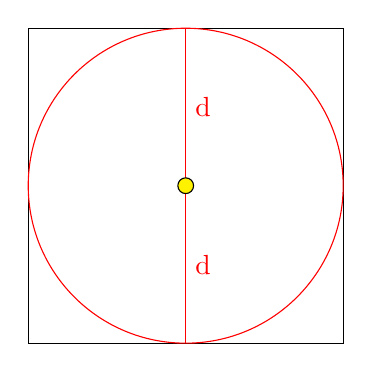
\begin{tikzpicture}
        \draw (-2,2) rectangle (2,-2);
        \draw[red] (0,2) -- (0,1) node[right]{d} -- (0,-1) node[right]{d} -- (0,-2);
        \draw[red] (0,0) circle(2);
        \draw[fill=yellow] (0,0) circle(0.1);
    \end{tikzpicture}
    \caption{跨越边界的范围}
\end{figure}

对于处于左边的每个点而言,在右边的每个小长方形中至多存在1个点,即最多只需要比较右边的6个点。如果在右半边存在超过6个点的话,那么就存在一个比d更短的距离,就与之前的最短距离矛盾了。 \\

\begin{figure}[H]
    \centering
    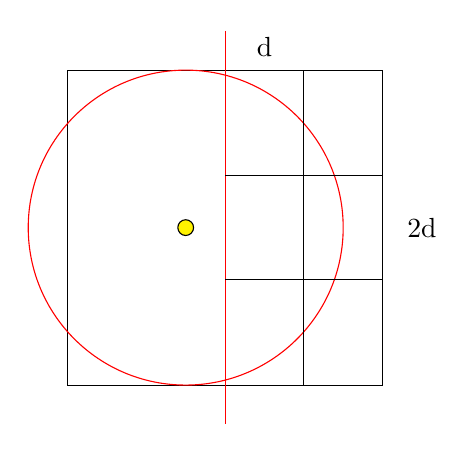
\begin{tikzpicture}
        \draw (-2,2) rectangle (2,-2);
        \draw[red] (0,2.5) -- (0,-2.5);
        \draw[red] (-0.5,0) circle(2);
        \draw[black] (0,0.66) -- (2,0.66);
        \draw[black] (0,-0.66) -- (2,-0.66);
        \draw[black] (1,2) -- (1,-2);
        \draw[fill=yellow] (-0.5,0) circle(0.1);
        \draw (0.5,2.3) node{d};
        \draw (2.5,0) node{2d};
    \end{tikzpicture}
    \caption{检查跨越边界的点}
\end{figure}

检查1个点是常数时间,检查n个点需要$ O(n) $的时间。分治算法中排序需要$ O(nlogn) $,递归处理子问题需要$ T(n/2) + O(n) $。总体时间复杂度为$ O(nlogn) $。

\newpage

\section{凸包}

\subsection{凸包(Convex Hull)}

凸包是计算几何中的概念。在大量离散点的集合中,求一个最小的凸多边形,使得所有点都在该多边形的内部或边上。凸包在形状识别、字形识别、碰撞检测中都有所应用。 \\

利用分治算法,连接最大纵坐标和最小纵坐标的两点,将点集划分成左右两部分,并递归对两个子问题进行求解。 \\

\begin{figure}[H]
    \centering
    \begin{tikzpicture}
        \filldraw (-1,4) circle (.1);
        \filldraw (0.5,3) circle (.1);
        \filldraw (-3,3) circle (.1);
        \filldraw (-4.3,2) circle (.1);
        \filldraw (-4,-1) circle (.1);
        \filldraw (-3,-3) circle (.1);
        \filldraw (3,4) circle (.1);
        \filldraw (4,2) circle (.1);
        \filldraw (2,-2.5) circle (.1);
        \draw (-3,-3)node[right]{$ y_{min} $} -- (3,4)node[right]{$ y_{max} $};
        \draw (0,0) node{d};
    \end{tikzpicture}
    \caption{划分点集}
\end{figure}

例如在左半边中,先找到距离边界d最远的点P。落在形成的三角形内部的点全部排除。接着将边a外的点与a构成作左半边点集的子问题,将边b外的点与b构成另一个左半边点集的子问题。每次将距离边界最远的点加入凸包即可求解原问题。 \\

\begin{figure}[H]
    \centering
    \begin{tikzpicture}
        \filldraw (-1,4) circle (.1);
        \filldraw (0.5,3) circle (.1);
        \filldraw (-3,3) circle (.1) node[left]{P};
        \filldraw (-4.3,2) circle (.1);
        \filldraw (-4,-1) circle (.1);
        \filldraw (-3,-3) circle (.1);
        \filldraw (3,4) circle (.1);
        \filldraw (4,2) circle (.1);
        \filldraw (2,-2.5) circle (.1);
        \draw (-3,-3)node[right]{$ y_{min} $} -- (3,4)node[right]{$ y_{max} $};
        \draw (0,0) node{d};

        \draw[red,dashed] (-3,3) -- (-3,-3) -- (-4,-1) -- (-4.2,2) -- (-3,3);
        \draw[blue,dashed] (-3,3) -- (3,4) -- (-1,4) -- (-3,3);
        \draw[red] (-2.7,0.5) node{a};
        \draw[blue] (0,3.2) node{b};
    \end{tikzpicture}
    \caption{子问题}
\end{figure}

每个子问题可以找到一个凸包上的点,使问题规模缩小1,寻找凸包顶点和划分子问题需要的时间$ O(n) $。当子问题的规模小于3时,可直接进行求解。因此分治算法的时间复杂度为:

\vspace{-0.5cm}

\begin{align*}
    W(n) = \begin{cases}
        O(1)            & n = 3 \\
        W(n - 1) + O(n) & n > 3
    \end{cases}
\end{align*}

求解得到:

\vspace{-0.5cm}

$$
    W(n) = O(n^2)
$$

\subsection{Graham扫描法}

Graham扫描法首先找到最靠近左下角的点,以这个点为极点,其它点按照极角排序。按照逆时针顺序进行扫描,先把点1压入凸包的栈中。 \\

